\chapter{Aufgaben 3}

\section{a)}

\textit{Welche technischen und rechtlichen Probleme sehen Sie bei der Auslagerung von
Datenverarbeitung in eine Cloud? Beschreiben Sie je ein Szenario, wo eine Auslagerung möglich bzw. nicht möglich ist.}\\

\noindent
Zu der Verarbeitung der Daten sollen diese an einen Cloud-Betreiber weitergegeben werden.
Es sind verschiedene Möglichkeiten denkbar, wie die Grundlage für die Datenverarbeitung gegeben ist (vgl.~\cite[60]{ITS6}):

\begin{itemize}
    \itemsep0.5em
    \item Software as a Service (SaaS): Der Cloud-Betreiber stellt Installation und Kapazitäten zur Verarbeitung der Daten über eine bestimmte Software zur Verfügung.
    Das Unternehmen muss sich um wenig kümmern, der Administrationsaufwand liegt beim Cloud-Betreiber.
    \item Platform as a Service (PaaS): Der Cloud-Betreiber stellt Installation und Kapazitäten zur Verfügung.
    Das Unternehmen muss sich um die Software zur Verarbeitung der Daten kümmern sowie um die Administration der betriebenen Anwendungen, die auf der Platform des Cloud-Anbieters laufen.
    \item Infrastructure as a Service (IaaS): Der Cloud-Betreiber stell Kapazitäten zur Verfügung.
    Das Unternehmen muss sich um die Administration der Betriebssysteme und aller Software kümmern, die auf den angemieteten Geräten des Cloud-Betreibers laufen.
\end{itemize}

\noindent
Wir können für jeden Fall festhalten: Der Cloud-Betreiber setzt Maßnahmen zur Erreichung des Schutzziels \textbf{Verfügbarkeit} um sowie allgemeine Maßnahmen zur Erreichung des Schutzziels \textbf{Vertraulichkeit} (Zugangskontrolle zu den Servern und der Netzwerkinfrastruktur).\\
Alle weiteren Schutzziele wie \textbf{Vertraulichkeit}, \textbf{Authentizität} sowie \textbf{Integrität} sind nur (oder ausschließlich bei SaaI) unter Mitwirkung des Unternehmens zu erreichen:

\begin{itemize}
    \itemsep0.5em
    \item Das Unternehmen trifft eine Entscheidung bei der Wahl der zu verwendenden Software.
    Dabei können Qualitätskriterien berücksichtigt werden, die zu der Erreichung o.g. Schutzziele dienen.
    \item Das Unternehmen selber ist die \Textit{Single-Source-of-Truth}\footnote{
    \url{https://en.wikipedia.org/wiki/Single_source_of_truth}, abgerufen 24.04.2025
    }: Die Daten werden auf Unternehmensseite generiert, die Analyse (und ggf. Archivierung, bspw. bei OLAP und einem Data Warehouse) findet in der Cloud statt.
    Das Unternehmen kommt nicht umhin, geeignete Schutzmaßnahmen seinerseits zu treffen, um Authentizität und Integrität der originären Daten sicherzustellen und mit dem Cloud-Anbieter \textbf{vertrauliche Datenkommunikation} zu vereinbaren und umzusetzen.
\end{itemize}

\noindent
Insgesamt wird das zu erreichende \textbf{Sicherheitsniveau} nach der Sensibilität und Geheimhaltungsstufen der verwendeten Daten beurteilt, was auch die Umsetzung der Auslagerung der Daten mitbestimmt: Es ist unmittelbar einleuchtend, das \textbf{rechtliche Probleme} entstehen können, wenn Daten kritischer Infrastrukturen an Cloud-Anbieter ausgelagert werden sollen, wenn es um die Übernahme der Verantwortung für die verschiedenen Schutzziele und mögliche damit einhergehende Schadensersatzforderungen geht.\\
Unter Umständen werden Cloud-Anbieter nicht bereit sein, im Auftrag von Behörden die technische und moralische Verantwortung zur Bewirtschaftung von Systemen mit personenbezogenen bzw. kritischen Daten unter Berücksichtigung des anzustrebenden Sicherheitsniveaus zu übernehmen, weil das Risiko zu hoch ist, dass der Cloud-Anbieter (und damit alle angeschlossenen Systeme verschiedenster Kunden) Ziel regelmäßiger Angriffe auf Infrastruktur und Daten wird.\\
Ein weiterer Aspekt sind die Garantien der Cloud-Betreiber hinsichtlich der Ausfallsicherheit: Je nach Rolle der verarbeiteten Daten und der damit verbundenen Geschäftsprozesse (z.B. Börsendaten im Finanzwesen) sind \textbf{Ausfallzeiten} in einem bestimmten Umfang nicht akzeptabel.

\noindent
Weitaus weniger Probleme entstehen, wenn die zu analysierenden Daten des Unternehmens anonymisiert sind:

\begin{itemize}
    \itemsep0.5em
    \item Daten können nicht auf Personen zurückgeführt werden
    \item Daten können durch den fehlenden Kontext nicht mit sicherheitskritischen oder wirtschaftlichen Fakten in Bezug gebracht werden
\end{itemize}

\noindent
In diesen Fällen kann davon ausgegangen werden, dass das Schutzziel \textbf{Vertraulichkeit} eher eine geringere Rolle spielt:
Geraten anonymisierte Daten in die Hände unbefugter, kann durch den fehlenden Kontext ein evtl. Schaden weitestgehend ausgeschlossen werden.
\textit{Schartner et al.} weisen in einen ähnlichen Zusammenhang~\cite[62]{ITS6} auf die Nutzung von \textit{Gruppen-Signaturen} hin, die dazu dienen können, der Erstellung von \textit{Nutzungsprofilen} entgegenzuwirken.
\noindent
Hängen allerdings weitere Faktoren von der Auswertung der Daten ab, und werden dadurch bspw. wirtschaftliche oder sonstige Entscheidungen abgeleitet, von denen Leib und Leben abhängen, muss in jedem Fall \textbf{Authentizität} und \textbf{Integrität} sichergestellt werden.

\noindent
Es lässt sich grob feststellen, dass eine Auslagerung in jedem Fall möglich ist, wenn die Daten wenig Schutzbedarf hinsichtlich Vertraulichkeit, Authentizität und Integrität benötigen.\\
Im anderen Fall müssen mit - ggfl. spezialisierten - Cloud-Betreibern geeignete Maßnahmen und SIS-Infrastrukturen zur Umsetzung der Schutzziele abgesprochen werden.
Diese Expertise kann auch dazu dienen, Cloud-Betreiber als technische Berater zur Umsetzung einer Unternehmensinternen Cloud-Infrastruktur heranzuziehen.\\

\noindent
In jedem Fall muss der Cloud-Betreiber \textbf{integer} sein, das Unternehmen muss dem Betreiber voll vertrauen können, bevor sensible Informationen und Daten ausgetauscht werden.
Das gilt letztendlich nicht nur für die Daten selber, sondern auch hinsichtlich der beim Cloud-Betreiber eingesetzter Software und den Verfahren, die dem besonderen Schutz des geistigen Eigentums des Unternehmens unterliegen.

\section{b)}

\textit{Wie können Sie sicherstellen, dass die Daten bei ihrer Verarbeitung in der Cloud
geschützt sind? Schlagen Sie diesbezüglich technische Lösungen vor und berücksichtigen Sie insbesondere die verschiedenen Varianten SaaS, IaaS und PaaS bei
Ihren Vorschlägen.}\\

\noindent
Die Verantwortung zum Schutz der Daten liegen sowohl bei dem Cloud-Anbieter, der die Daten zur Verabeitung entgegennimmt, als auch dem Unternehmen, das die Daten zur Verfügung stellt.
Je nach Dienstmodell sind die Verantwortlichkeiten anders gewichtet.
Allgemein kann zunächst festgestellt werden:

\noindent
Das Unternehmen vereinbart mit dem Cloud-Betreiber eine sichere Datenverbindung zur \textbf{vertraulichen} Übertragung der Daten.
Es werden die übliche Maßnahmen zur Verifikation der öffentlichen Schlüssel der an der Kommunikation beteiligten Systeme getroffen, und zwar mit Hilfe einer übergeordneten Vertrauensinstanz (\textit{Certification Authority}) und einer geeigneten SIS, wodurch \textbf{Authentizität} und \textbf{Integrität} sichergestellt werden soll.\\

\noindent
Das Unternehmen stellt sicher, dass die Daten gesammelt werden, damit sie zur Verarbeitung an den Cloud-Anbieter gesendet werden können.\\
Findet eine Archivierung der Daten \textit{bei dem Unternehmen} statt, sorgt das Unternehmen für geeignete technische Maßnahmen, u.a. auch für geeignetes Notfallvorsorge-Konzept (Backup-Strategie).\\
Der Cloud-Betreiber sorgt dafür, dass die Auswertung der Daten für das Unternehmen zur Verfügung gestellt werden.
Werden Daten bei dem Cloud-Anbieter archiviert, ergreift der Cloud-Anbieter entsprechende Schutzmaßnahmen zur Sicherung der Daten.
Diese Schritte dienen zur Sicherstellung der \textbf{Verfügbarkeit} der Daten, wobei hier vor allem dem Cloud-Anbieter eine tragende Rolle zukommen, der letztendlich Kapazitäten und die Infrastruktur für die Verarbeitung der Daten bereitstellt.
Diese müssen durch den Cloud-Anbieter abgesichert werden, wobei die üblichen technischen und organisatorischen Maßnahmen anzuwenden sind, die letztliche alle Dienstmodelle betreffen, darunter u.a.:

\begin{itemize}
    \itemsep0.5em
    \item \textbf{Verschlüsselung} der verarbeiteten Daten, sofern diese nicht anonymisiert sind.
    \item \textbf{Firewalls} und \textbf{Proxies} zur Absicherung interner Systeme.
    \item \textbf{IPS} und \textbf{IDS} zur Prävention und Detektion von Angriffen.
    \item \textbf{Sicherheitsbeauftragte} zur Steuerung und Kommunikation von Maßnahmen, die der Wahrung der Schutzziele dienen.
    \item Personal, das über eine hohe (sicherheits)technische Expertise verfügt, und das mit dem Einspielen von Patches und der Aktualisierung von Software vertraut ist, gerade bei den Dienstmodellen \textit{SaaS} und \textit{PaaS}.
\end{itemize}

\noindent
Wie in Aufgabenteil a) festgestellt, liegt vor allem bei bei dem Unternehmen bei dem Dienstmodell \textit{IaaS} eine hohe Verantwortung bzgl. der Erreichung der Schutzziele, da die Administration der auf der vom Cloud-Betreiber zur Verfügung gestellten Infrastruktur durch das Unternehmen erfolgen muss.
Hierzu gehören auch kryptografische Maßnahmen, wie die o.a. Verschlüsselung der verarbeiteten Daten, sofern notwendig.\\
Betrachten wir hingegen \textit{SaaS}, kommt dem Unternehmen vergleichsweise wenig Verantwortung bei der Absicherung der Daten zu, da die beteiligten Systemkomponenten weitestgehend durch den Cloud-Anbieter betreut und administriert werden.
Wie bei \textit{Paas} gehören hierzu auch \textbf{Zugriffskontrollen} und \textbf{Rechte-/Rollenverteilung} für die eingesetzten Softwarekomponenten.


\section{c)}

\textit{Entwerfen und beschreiben Sie ein Zugriffs-Kontrollsystem einschließlich KeyManagement, welches Ihre Daten vor unberechtigtem Zugriff durch den CloudProvider schützt.}\\

\noindent
Die Abbildung~\ref{fig:cloudkomm} stellt schematisch den Ablauf der Kommunikation zwischen einem System $SysB$, das bei dem Cloud-Betreiber $B$ betrieben wird, und dem Unternehmen $A$ unter Einsatz einer \textit{Certification Authority} dar.
Die CA sorgt für die Zertifizierung der öffentlichen Schlüssel von $A$ und $SysB$: Bei der Datenkommunikation können die übermittelten Zertifikate von der CA überprüft und nach kryptografischer Verifikation einem Besitzer eindeutig zugeordnet werden.

\begin{figure}
    \centering
    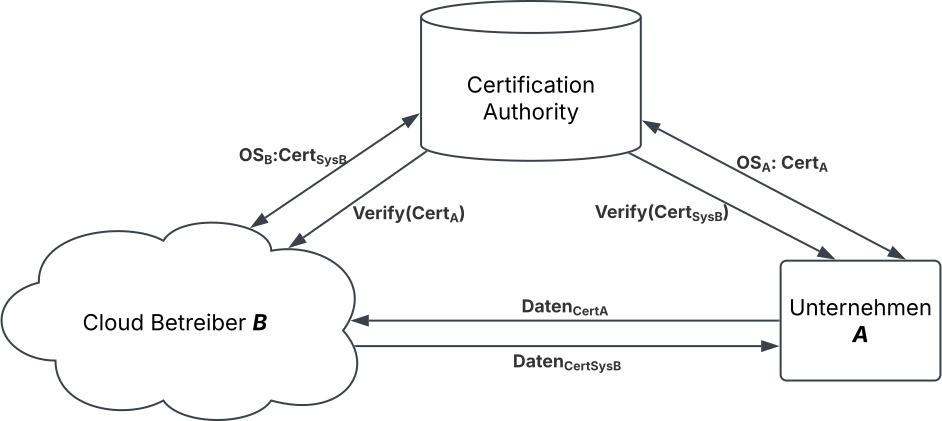
\includegraphics[scale=0.4]{aufgabe 3/img/cloudkomm.svg}
    \caption{Schematische Darstellung vertraulicher Kommunikation zwischen einem System eines Cloud-Anbieters und Unternehmen unter Einsatz einer \textit{Certification Authority}, wodurch auch Integrität und Authentizität sichergestellt werden soll. (Quelle: eigene)}
    \label{fig:cloudkomm}
\end{figure}

\noindent
Die Zertifikate werden bei Verbindungsaufbau ausgetauscht und für die Kommunikation innerhalb dieser Sitzung - bspw. unter Anwendung von SSL/TLS\footnote{
\textit{Transport Layer Security} / \textit{Secure Sockets Layer}
} - verwendet, um Authentizität, Vertraulichkeit und Integrität der ausgetauschten Daten zu garantieren.
Hierzu wird bei Anwendung hybrider Verschlüsselung noch ein symmetrischer Sitzungsschlüssel vereinbart.\\
Da der Cloud-Betreiber selber nicht im Besitz der privaten Schlüssel von $SysB$ ist, sind die übertragenen Daten vor ihm verborgen\footnote{
Je nach angebotener Software bei dem Dienstmodell \textit{SaaS} muss hier ggfl. auf ein anderes Dienstmodell (oder einen anderen Anbieter, dessen eingesetzte Software die Arbeit mit verschlüsselten Daten erlaubt) gewechselt werden.
}.